\documentclass[12pt,a4paper]{article}

\usepackage[utf8]{inputenc}
\usepackage[T1]{fontenc}
\usepackage[french]{babel}
\usepackage{lmodern}
\usepackage{geometry}
\geometry{margin=2.4cm}
\usepackage{amsmath,amssymb}
\usepackage{booktabs}
\usepackage{graphicx}
\usepackage{float}
\usepackage{array}
\usepackage{longtable}
\usepackage{enumitem}
\usepackage{xcolor}
\usepackage{listings}
\usepackage{hyperref}
\usepackage{microtype}
\usepackage{fancyhdr}

\hypersetup{
  colorlinks=true,
  linkcolor=black,
  citecolor=black,
  urlcolor=blue
}

\setlength{\headheight}{15pt}
\pagestyle{fancy}
\fancyhf{}
\lhead{TP Science de données}
\rhead{Nuées dynamiques}
\cfoot{\thepage}

\lstset{
  language=Python,
  basicstyle=\ttfamily\small,
  breaklines=true,
  frame=single,
  showstringspaces=false,
  columns=fullflexible,
  keywordstyle=\bfseries,
  commentstyle=\itshape,
  literate={é}{{\'e}}1 {è}{{\`e}}1 {ê}{{\^e}}1 {ë}{{\"e}}1 {à}{{\`a}}1 {â}{{\^a}}1 {ù}{{\`u}}1 {û}{{\^u}}1 {ü}{{\"u}}1 {ô}{{\^o}}1 {ö}{{\"o}}1 {î}{{\^i}}1 {ï}{{\"i}}1 {ç}{{\c{c}}}1 {É}{{\'E}}1 {È}{{\`E}}1 {Ê}{{\^E}}1 {À}{{\`A}}1 {Ù}{{\`U}}1 {Û}{{\^U}}1
}

\newcommand{\etudiant}{BETSHINDO NDJAMBE CHRISTENVIE}
\newcommand{\sujet}{Implémentation de l'algorithme des Nuées Dynamiques (from scratch)}

\begin{document}
\pagenumbering{gobble}

\begin{titlepage}
\centering
\thispagestyle{empty}

{\Large\bfseries UNIVERSITÉ DE KINSHASA\par}
\vspace{0.25cm}
{\large\bfseries FACULTÉ DES SCIENCES ET TECHNOLOGIES\par}
\vspace{0.2cm}
{\normalsize MASTER 1, MATHÉMATIQUES, STATISTIQUE ET INFORMATIQUE (MSI)\par}

\vspace{0.9cm}

\includegraphics[width=4.4cm]{logo_unikin.png}

\vspace{0.9cm}
{\Large\bfseries TRAVAUX PRATIQUES\par}
\vspace{0.15cm}
{\large SCIENCE DES DONNÉES\par}

\vspace{1.2cm}
\rule{0.92\textwidth}{0.8pt}\par
\vspace{0.45cm}
{\LARGE\bfseries IMPLÉMENTATION DE L'ALGORITHME\par}
\vspace{0.22cm}
{\LARGE\bfseries DES NUÉES DYNAMIQUES\par}
\vspace{0.45cm}
\rule{0.92\textwidth}{0.8pt}\par

\vfill
\begin{flushleft}
{\large\bfseries PAR :}\par
\vspace{0.25cm}
{\large \etudiant}\par
\end{flushleft}

\vfill
{\large\bfseries SEPTEMBRE 2026\par}
\end{titlepage}
\pagenumbering{arabic}

\tableofcontents
\newpage

\section{Résumé}

Ce travail présente une implémentation \textit{from scratch} d'un cadre de classification inspiré de la méthode des Nuées Dynamiques introduite par Edwin Diday en 1971 pour la classification automatique et la reconnaissance des formes \cite[pp.~19--21]{diday1971}. Le principe historique repose sur une alternance entre l'affectation des individus aux classes et la mise à jour d'éléments représentatifs, appelés étalons, jusqu'à stabilisation \cite[p.~21]{diday1971}.

L'application développée dans ce TP généralise volontairement la notion de représentant au niveau logiciel. L'utilisateur choisit entre cinq modes : un point unique, plusieurs points représentatifs, des axes principaux, une distribution gaussienne et une structure robuste fondée sur la médiane et la MAD. Les trois derniers modes sont des extensions de conception du TP et ne sont pas présentés comme des variantes explicitement programmées dans l'article de Diday. Les concepts utilisés pour ces extensions sont documentés par des références propres : k-means \cite{macqueen1967,lloyd1982}, analyse en composantes principales \cite{jolliffe2016}, distance quadratique de Mahalanobis \cite{mahalanobis1936}, estimation robuste par MAD \cite{rousseeuwcroux1993}.

Le moteur de clustering, les distances, la silhouette et l'Adjusted Rand Index ont été programmés directement, sans appel à un algorithme de clustering de \texttt{scikit-learn}. NumPy est utilisé uniquement pour les opérations numériques et l'algèbre linéaire \cite{harris2020}. Les résultats expérimentaux et les figures présentés dans ce rapport proviennent de l'exécution du code fourni avec ce TP ; leur origine est indiquée explicitement comme « calculs de l'auteur ».

\section{Traçabilité des sources et prévention du plagiat}

Afin d'éviter toute confusion entre les idées de la littérature et les choix propres au TP, nous appliquons la règle suivante : tout concept, algorithme, métrique ou résultat théorique emprunté à une source externe est reformulé et accompagné d'une citation ; tout élément conçu spécifiquement pour ce projet est signalé comme un choix de conception ou un calcul de l'auteur. Aucun paragraphe théorique n'est volontairement reproduit mot pour mot depuis une source.

\begin{longtable}{p{4.0cm}p{5.3cm}p{5.0cm}}
\caption{Table de traçabilité scientifique des principaux éléments du projet.}\\
\toprule
\textbf{Élément} & \textbf{Référence scientifique} & \textbf{Statut dans ce TP} \\
\midrule
\endfirsthead
\toprule
\textbf{Élément} & \textbf{Référence scientifique} & \textbf{Statut dans ce TP} \\
\midrule
\endhead
Méthode des Nuées Dynamiques & Diday (1971) \cite{diday1971} & Base historique et cycle itératif \\
Représentants multiples / étalons & Diday (1971) \cite[p.~25]{diday1971} & Adaptation directe de l'idée des étalons \\
Centroïde / k-means & MacQueen (1967), Lloyd (1982) \cite{macqueen1967,lloyd1982} & Cas ponctuel de notre architecture \\
Initialisation probabiliste & Arthur et Vassilvitskii (2007) \cite{arthur2007} & Initialisation inspirée de k-means++ \\
Sélection éloignée de prototypes & Gonzalez (1985) \cite{gonzalez1985} & Inspiration pour l'initialisation farthest-first \\
Échange local de prototypes & Kaufman et Rousseeuw (1990) \cite{kaufman1990} & Raffinement de type médoïde, simplifié \\
Axes principaux & Jolliffe et Cadima (2016) \cite{jolliffe2016} & Extension du TP par ACP locale \\
Distance quadratique / covariance & Mahalanobis (1936) \cite{mahalanobis1936} & Composante de la représentation gaussienne \\
Médiane et MAD & Rousseeuw et Croux (1993) \cite{rousseeuwcroux1993} & Extension robuste du TP \\
Silhouette & Rousseeuw (1987) \cite{rousseeuw1987} & Métrique d'évaluation \\
Adjusted Rand Index & Hubert et Arabie (1985) \cite{hubert1985} & Métrique d'évaluation externe \\
Calcul numérique & Harris et al. (2020) \cite{harris2020} & NumPy pour tableaux et algèbre linéaire \\
\bottomrule
\end{longtable}

\noindent\textit{Source du tableau : synthèse de l'auteur à partir des références citées.}

\section{Introduction}

La classification non supervisée vise à construire des groupes à partir des seules observations, sans étiquettes de classes fournies à l'algorithme. Dans l'article fondateur des Nuées Dynamiques, Diday formule le problème en recherchant des groupes dont les individus sont aussi semblables que possible à l'intérieur d'une classe et aussi différents que possible entre classes \cite[p.~20]{diday1971}. Cette formulation s'inscrit dans le cadre général de l'analyse de groupes et de la classification automatique \cite{kaufman1990}.

Les méthodes de type k-means représentent chaque classe par un centre obtenu à partir des observations qui lui sont affectées ; dans la version classique, l'algorithme alterne entre une étape d'affectation au centre le plus proche et une étape de recalcul des centres \cite{macqueen1967,lloyd1982}. Cette représentation ponctuelle est simple, mais elle ne décrit pas explicitement la forme interne d'un groupe lorsqu'une seule moyenne est insuffisante.

Diday propose au contraire d'associer à une classe plusieurs objets représentatifs, appelés étalons, et de définir une distance entre un individu et cet ensemble \cite[pp.~20--21]{diday1971}. Dans l'exemple artificiel de son article, l'utilisation de nombreux étalons permet de suivre la géométrie de formes allongées, alors qu'un unique centre de gravité donnerait une description plus arrondie de ces formes \cite[p.~25]{diday1971}. Ce constat motive l'architecture modulaire de notre application.

Dans ce TP, le cycle général de Diday est conservé, mais la notion de représentant est rendue interchangeable. Les modes « axes », « distribution » et « structure robuste » constituent des extensions réalisées pour répondre au cahier des charges pédagogique ; leurs formules et leurs fondements sont référencés séparément dans les sections suivantes.

\section{Fondements théoriques}

\subsection{Formulation de Diday}

Soit $E=\{x_1,\ldots,x_N\}$ l'ensemble des individus à classer. Diday introduit une collection de $K$ ensembles représentatifs $E_i$, chacun contenant $n_i$ objets, ainsi qu'une fonction $D$ mesurant la proximité entre un individu et un ensemble de représentants \cite[p.~20]{diday1971}. Dans notre notation, une partition des observations est écrite
\[
\mathcal{C}=\{C_1,C_2,\ldots,C_K\},
\]
et la collection des représentations est notée
\[
L=(E_1,E_2,\ldots,E_K).
\]

L'algorithme historique calcule $D(x,E_i)$ pour chaque observation et chaque classe, construit les classes à partir de ces distances, puis met à jour les étalons en minimisant une fonction d'agrégation--écartement $R(x,i,L)$ \cite[p.~21]{diday1971}. Une écriture synthétique du cycle est donc :

\begin{enumerate}[label=\arabic*)]
    \item initialiser les ensembles représentatifs ;
    \item calculer les coûts ou distances de chaque observation vers chaque classe ;
    \item affecter les observations aux classes ;
    \item mettre à jour les représentants selon le critère choisi ;
    \item répéter jusqu'à stabilisation.
\end{enumerate}

Cette liste est une reformulation pédagogique des étapes de la section III.2 de Diday \cite[p.~21]{diday1971}. L'article indique également comme paramètres d'entrée le tableau de données, le nombre maximal de classes $K$ et le nombre d'étalons par classe ; sans information préalable, les étalons initiaux peuvent être choisis aléatoirement \cite[p.~23]{diday1971}.

\subsection{Convergence dans le cadre original}

Diday définit un « élément améliorant », une notion d'optimum local et une condition de convergence pour la suite des représentations \cite[p.~22]{diday1971}. Il établit ensuite que, sous une propriété particulière de la fonction $R$ appelée « carrée », la suite converge vers un optimum local \cite[p.~23]{diday1971}. L'auteur précise aussi qu'en pratique la méthode est souvent observée comme convergente même lorsque cette condition suffisante n'est pas satisfaite \cite[p.~23]{diday1971}.

Les extensions de notre TP ne reprennent pas toutes exactement la fonction $R$ du cadre historique. Notre programme utilise donc deux critères pratiques d'arrêt : stabilité des étiquettes et faible variation relative du critère numérique. \textit{Ces deux critères sont des choix d'implémentation de l'auteur et ne sont pas présentés comme le théorème de convergence de Diday.}

\subsection{Cas ponctuel et lien avec k-means}

Dans le mode \texttt{point}, chaque classe $C_i$ est représentée par sa moyenne :
\[
\mu_i = \frac{1}{|C_i|}\sum_{x\in C_i}x.
\]
L'affectation utilise la distance euclidienne au carré
\[
d_i(x)=\|x-\mu_i\|_2^2.
\]
La répétition des étapes « affectation au centre le plus proche » puis « recalcul de la moyenne » correspond au schéma classique associé à k-means \cite{macqueen1967,lloyd1982}. Dans notre architecture, k-means apparaît donc comme le cas où la représentation de chaque classe est réduite à un seul point. Il s'agit ici d'une observation sur le comportement du code développé, et non d'une citation textuelle de Diday.

\section{Représentations proposées dans l'application}

\subsection{Représentation par un point}

Le représentant est le centroïde de la classe et le coût est la distance euclidienne au carré. Cette formulation est celle du cas k-means décrit précédemment \cite{macqueen1967,lloyd1982}. \textit{L'intégration de ce mode dans l'interface commune des Nuées Dynamiques est un choix d'architecture de l'auteur.}

\subsection{Représentation par plusieurs points}

Diday appelle « étalons » les éléments représentatifs d'une classe et montre l'intérêt de plusieurs étalons pour épouser une géométrie non ponctuelle \cite[pp.~21,25]{diday1971}. Dans notre implémentation, une classe est décrite par
\[
P_i=\{p_{i1},\ldots,p_{im}\},
\]
où les prototypes sont des observations réelles de la classe.

L'initialisation des prototypes adopte une stratégie de couverture de type \textit{farthest-first}, apparentée à l'idée d'ajouter successivement un point éloigné des représentants déjà sélectionnés \cite{gonzalez1985}. Un raffinement local par échanges de prototypes est ensuite utilisé ; cette logique est inspirée des méthodes à médoïdes telles que PAM, mais elle est volontairement simplifiée dans ce TP \cite{kaufman1990}. Le coût d'affectation proposé est soit
\[
d_i(x)=\min_j \|x-p_{ij}\|_2^2,
\]
soit la moyenne des distances aux prototypes. \textit{Le choix entre minimum et moyenne est un paramètre propre à notre implémentation.}

\subsection{Représentation par axes factoriels}

L'analyse en composantes principales recherche des directions orthogonales maximisant successivement la variance, et ces directions peuvent être obtenues par un problème de valeurs propres de la matrice de covariance \cite{jolliffe2016}. Dans notre extension, chaque classe est représentée par un centre $\mu_i$ et un ensemble de $q$ directions principales $U_i$ calculées uniquement sur les observations de cette classe.

Pour $x$, nous projetons $x-\mu_i$ sur le sous-espace porté par $U_i$. Le résidu orthogonal est
\[
r=x-\mu_i-U_iU_i^\top(x-\mu_i).
\]
Nous définissons ensuite le coût
\[
d_i(x)=\|r\|_2^2+\alpha\|U_i^\top(x-\mu_i)\|_2^2.
\]
La première partie mesure l'écart au sous-espace principal ; le second terme, pondéré par un petit $\alpha$, a été ajouté par l'auteur pour départager certaines configurations où plusieurs axes donnent des distances orthogonales très proches. \textit{Cette fonction de coût exacte est donc une construction du TP, fondée sur l'ACP mais non reprise telle quelle d'une source.}

\subsection{Représentation par une distribution de probabilités}

Une distribution gaussienne multivariée est caractérisée par une moyenne $\mu_i$ et une matrice de covariance $\Sigma_i$. La forme quadratique
\[
(x-\mu_i)^\top\Sigma_i^{-1}(x-\mu_i)
\]
est liée à la distance généralisée introduite par Mahalanobis \cite{mahalanobis1936}. En tenant compte du volume de la covariance, notre coût devient
\[
d_i(x)=(x-\mu_i)^\top\Sigma_i^{-1}(x-\mu_i)+\log|\Sigma_i|.
\]
À une constante commune près, cette expression correspond au terme dépendant de la classe dans la log-vraisemblance négative d'une densité gaussienne multivariée. Une régularisation $\lambda I$ est ajoutée avant inversion pour traiter les covariances mal conditionnées. \textit{Le choix de cette représentation comme extension des Nuées Dynamiques est propre au TP ; la formule s'appuie sur les propriétés classiques de la loi gaussienne multivariée et de la distance de Mahalanobis} \cite{mahalanobis1936}.

\subsection{Structure représentative robuste}

Pour illustrer le cas d'une « structure représentative » non réduite à un point ou à une covariance, nous utilisons un couple centre-échelle robuste. La médiane est calculée variable par variable et l'échelle utilise la MAD. Rousseeuw et Croux rappellent notamment l'usage du facteur $1.4826$ pour rendre la MAD cohérente avec l'écart-type sous une hypothèse gaussienne \cite{rousseeuwcroux1993}. Notre représentant est donc
\[
\widetilde{\mu}_{ij}=\operatorname{median}(x_j),
\qquad
s_{ij}=1.4826\,\operatorname{median}(|x_j-\widetilde{\mu}_{ij}|)+\varepsilon,
\]
et le coût choisi est
\[
d_i(x)=\sum_j\left|\frac{x_j-\widetilde{\mu}_{ij}}{s_{ij}}\right|.
\]
La combinaison précise « médiane + MAD + somme des écarts normalisés » est un exemple d'architecture conçu pour ce TP ; elle n'est pas attribuée à Diday ni à Rousseeuw et Croux.

\paragraph{Positionnement méthodologique.}
L'article de 1971 formalise explicitement des ensembles d'étalons, ainsi que des fonctions générales $D$ et $R$ \cite[pp.~20--21]{diday1971}. Les modes « axes », « distribution » et « structure robuste » sont donc des extensions logicielles documentées par leurs propres références scientifiques. Cette distinction est maintenue dans tout le rapport afin de ne pas attribuer à l'article historique des éléments qui n'y figurent pas.

\section{Architecture de l'implémentation}

Le projet est organisé en modules indépendants. \textit{L'organisation logicielle décrite ci-dessous est une conception originale du projet et n'est pas extraite d'une source externe.}

\begin{verbatim}
.
|-- app.py
|-- streamlit_app.py
|-- src/
|   |-- dynamic_clouds.py
|   |-- representations.py
|   |-- metrics.py
|   `-- data.py
|-- experiments/run_experiments.py
|-- tests/test_dynamic_clouds.py
`-- report/rapport.tex
\end{verbatim}

Le fichier \texttt{dynamic\_clouds.py} contient la boucle d'affectation et de mise à jour. Le fichier \texttt{representations.py} définit une interface commune avec deux opérations : \texttt{fit(X\_cluster)} pour mettre à jour un représentant et \texttt{cost(X)} pour calculer les coûts d'affectation. Cette séparation permet au moteur de conserver le même cycle général malgré des représentants de nature différente. NumPy fournit les tableaux, produits matriciels, valeurs propres et routines numériques utilisées par ces modules \cite{harris2020}.

\subsection{Pseudo-code général}

Le pseudo-code suivant est une synthèse du programme écrit pour ce TP ; son alternance « affectation / mise à jour » s'inspire du cycle de Diday \cite[p.~21]{diday1971}, tandis que les détails d'arrêt et de réparation des classes vides sont propres à notre implémentation.

\begin{lstlisting}[language={},caption={Pseudo-code du moteur développé. Source : conception de l'auteur à partir du cycle général de Diday \cite{diday1971}.}]
Entrée : X, K, type_representation, paramètres
Initialiser une partition en K classes non vides
Construire un représentant pour chaque classe

Pour t = 1, ..., max_iter :
    Pour chaque classe i :
        calculer le coût d_i(x) pour tous les x
    Affecter chaque x à la classe de coût minimal
    Réparer les éventuelles classes vides
    Calculer le critère global
    Mettre à jour chaque représentant avec sa nouvelle classe

    Si les étiquettes ne changent plus
       ou si la variation relative <= tolérance :
        arrêter

Retourner la partition, les représentants et l'historique du critère
\end{lstlisting}

\subsection{Initialisation}

Pour limiter les démarrages défavorables, le code sélectionne les graines selon une règle inspirée de k-means++, où la probabilité de choisir un nouveau centre dépend de sa distance aux centres déjà choisis \cite{arthur2007}. Notre implémentation est écrite directement en NumPy et n'appelle pas une fonction externe de k-means++. Ce choix diffère de l'initialisation aléatoire des étalons mentionnée par Diday lorsque l'utilisateur ne dispose pas d'information a priori \cite[p.~23]{diday1971}.

\subsection{Gestion des classes vides}

Diday signale que des classes vides peuvent apparaître lorsque le nombre demandé de classes est trop grand par rapport à la structure effectivement présente dans les données \cite[p.~25]{diday1971}. Dans notre programme, une classe devenue vide est réparée en lui réaffectant une observation parmi les moins bien représentées, sans vider la classe d'origine. \textit{La stratégie précise de réparation est une décision d'implémentation de l'auteur.}

\section{Complexité}

Les ordres de grandeur ci-dessous sont déduits directement des boucles et opérations matricielles de notre code. Ils ne constituent pas un théorème repris d'une publication. Diday discute déjà le coût des calculs de $D(x,E_k)$ et de $R(x,i,L)$ et souligne l'intérêt d'éviter la conservation de toutes les distances deux à deux \cite[p.~24]{diday1971}, mais les variantes modernes de notre application ont des coûts propres.

Soient $N$ le nombre d'individus, $d$ le nombre de variables, $K$ le nombre de classes, $m$ le nombre de prototypes et $q$ le nombre d'axes.

\begin{table}[H]
\centering
\caption{Ordres de grandeur par itération. Source : analyse du code par l'auteur.}
\begin{tabular}{p{3.4cm}p{8.3cm}}
\toprule
\textbf{Représentation} & \textbf{Coût dominant approximatif} \\
\midrule
Point & $O(NKd)$ pour les distances et les moyennes \\
Plusieurs points & $O(NKmd)$ pour l'affectation, plus le raffinement local des prototypes \\
Axes & $O(NKdq)$ pour l'affectation, plus les décompositions propres des covariances \\
Distribution & $O(NKd^2)$ pour les formes quadratiques, plus $O(Kd^3)$ pour les opérations sur covariance \\
Structure robuste & $O(NKd)$ pour les distances normalisées \\
\bottomrule
\end{tabular}
\end{table}

\section{Expérimentation}

\subsection{Jeu de données}

Un jeu synthétique bidimensionnel de 360 observations a été généré spécifiquement pour le TP avec trois groupes de géométries différentes. Les données et les étiquettes de référence sont produites par le script \texttt{experiments/run\_experiments.py}. \textit{Il s'agit donc de données synthétiques de l'auteur, et non d'un jeu recopié d'une publication.}

\begin{figure}[H]
\centering
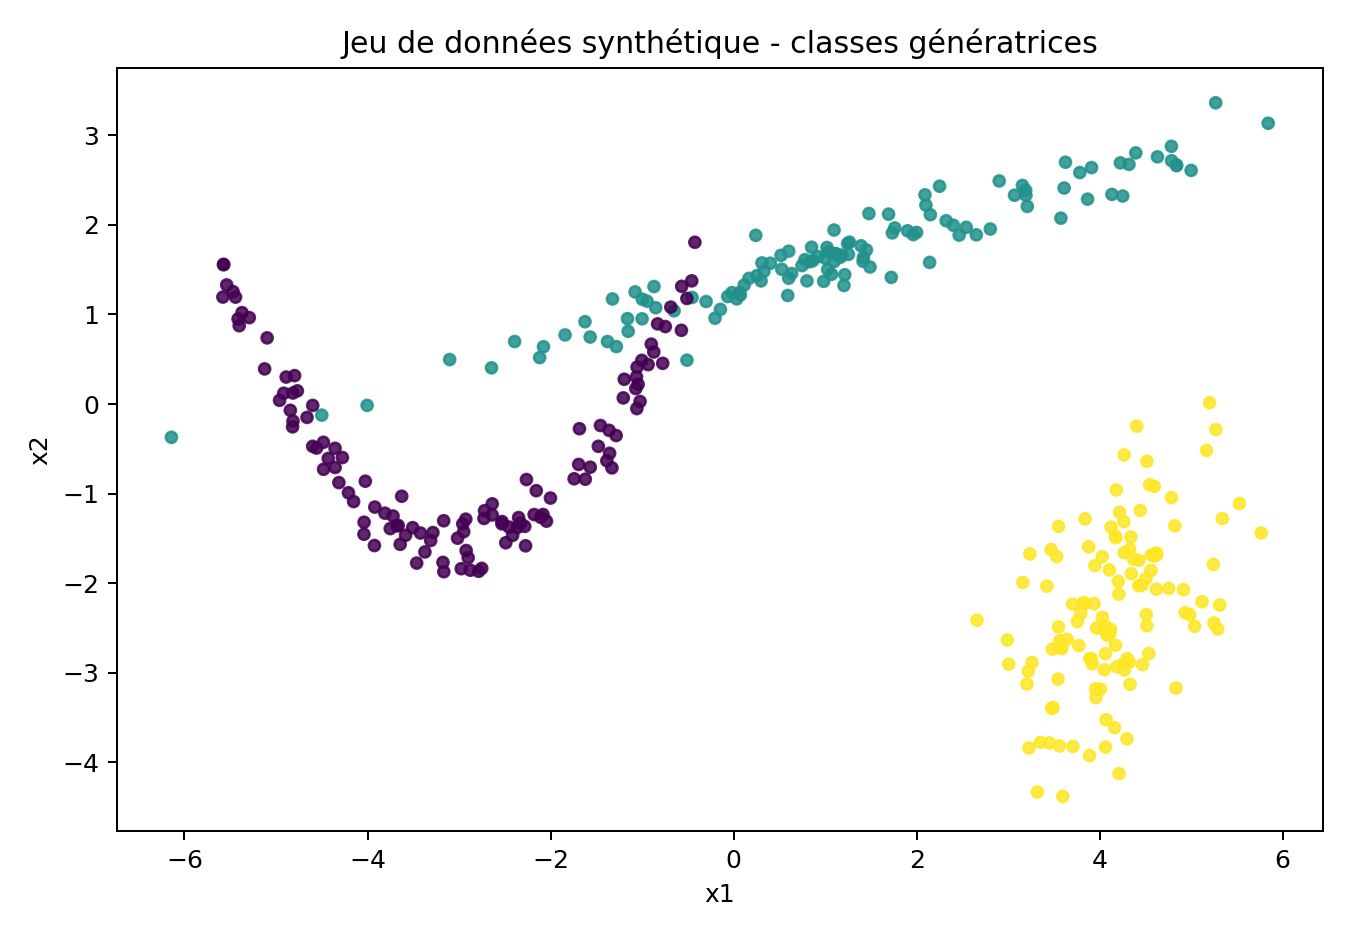
\includegraphics[width=0.72\textwidth]{figures/dataset.png}
\caption{Jeu synthétique utilisé pour l'évaluation. Source : génération par le code de l'auteur.}
\end{figure}

\subsection{Protocole et métriques}

Chaque variante est exécutée avec $K=3$ et une graine aléatoire fixe pour rendre l'expérience reproductible. Le mode multi-points utilise sept prototypes par classe et le mode axes un axe principal. \textit{Ces valeurs sont des choix expérimentaux de l'auteur.}

Le coefficient de silhouette compare, pour chaque observation, la cohésion avec sa propre classe et la séparation par rapport aux autres classes ; la moyenne des silhouettes peut servir à apprécier une partition \cite{rousseeuw1987}. L'Adjusted Rand Index compare deux partitions tout en corrigeant l'accord attendu par hasard \cite{hubert1985}. Les deux métriques sont recodées dans \texttt{src/metrics.py} à partir de leurs définitions, sans appel à \texttt{sklearn.metrics}.

Le critère interne de chaque représentation est également enregistré. Comme les cinq modes n'utilisent pas la même fonction de coût, leurs valeurs brutes ne sont pas interprétées comme une échelle commune. \textit{Cette précaution d'interprétation découle de la conception du programme.}

\subsection{Résultats}

\begin{table}[H]
\centering
\caption{Résultats sur le jeu synthétique. Source : calculs de l'auteur obtenus par \texttt{run\_experiments.py}.}
\begin{tabular}{lrrrr}
\toprule
\textbf{Représentation} & \textbf{Itérations} & \textbf{Silhouette} & \textbf{ARI} & \textbf{Convergence} \\
\midrule
Point & 3 & 0.621 & 0.833 & Oui \\
Plusieurs points & 4 & 0.613 & 0.794 & Oui \\
Axes & 8 & 0.595 & 0.758 & Oui \\
Distribution & 3 & 0.615 & 0.875 & Oui \\
Structure robuste & 6 & 0.588 & 0.755 & Oui \\
\bottomrule
\end{tabular}
\end{table}

Sur ce jeu synthétique précis, la distribution obtient l'ARI le plus élevé, tandis que le mode ponctuel obtient la silhouette la plus élevée. Ces nombres décrivent uniquement cette exécution et ne constituent pas une conclusion universelle sur les méthodes. La silhouette est interprétée conformément à sa définition de validation de partitions \cite{rousseeuw1987}, tandis que l'ARI mesure ici l'accord avec les étiquettes synthétiques connues \cite{hubert1985}.

\begin{figure}[H]
\centering
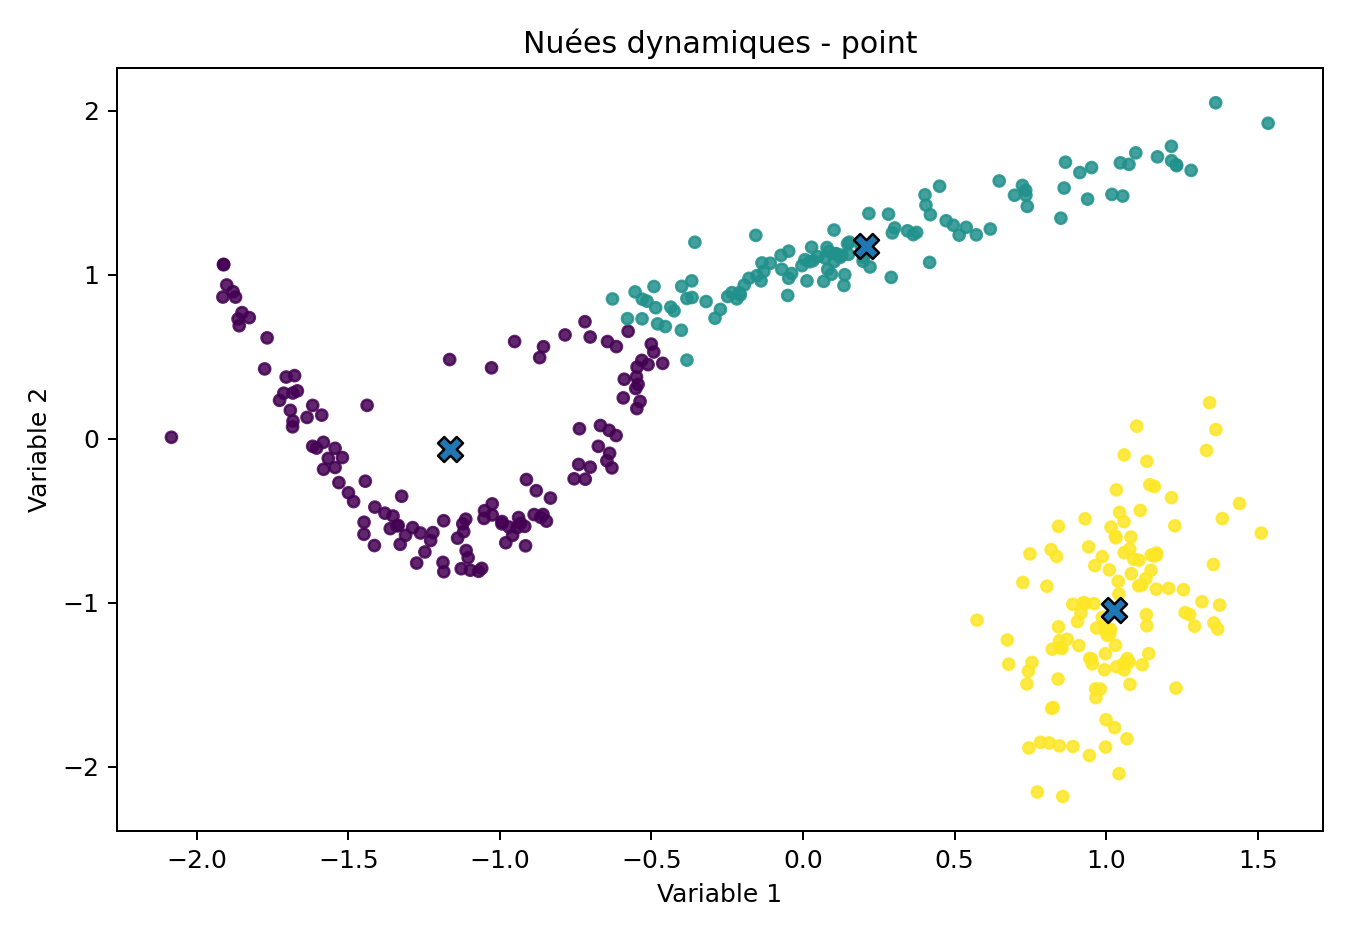
\includegraphics[width=0.72\textwidth]{figures/partition_point.png}
\caption{Partition avec un point par classe. Source : calculs et visualisation de l'auteur.}
\end{figure}

\begin{figure}[H]
\centering
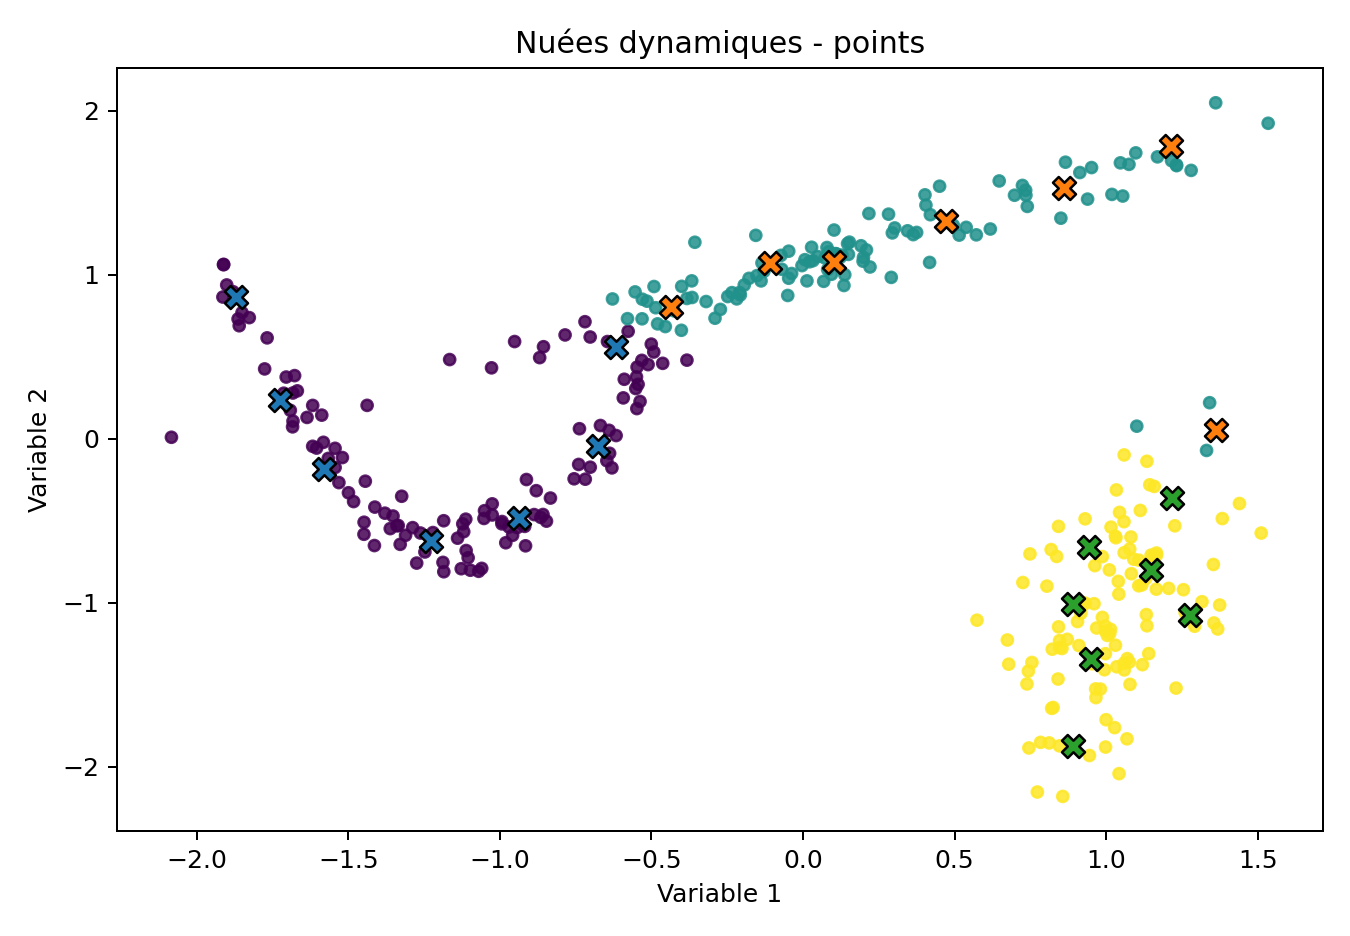
\includegraphics[width=0.72\textwidth]{figures/partition_points.png}
\caption{Partition avec plusieurs points représentatifs ; les croix indiquent les prototypes. Source : calculs et visualisation de l'auteur.}
\end{figure}

\begin{figure}[H]
\centering
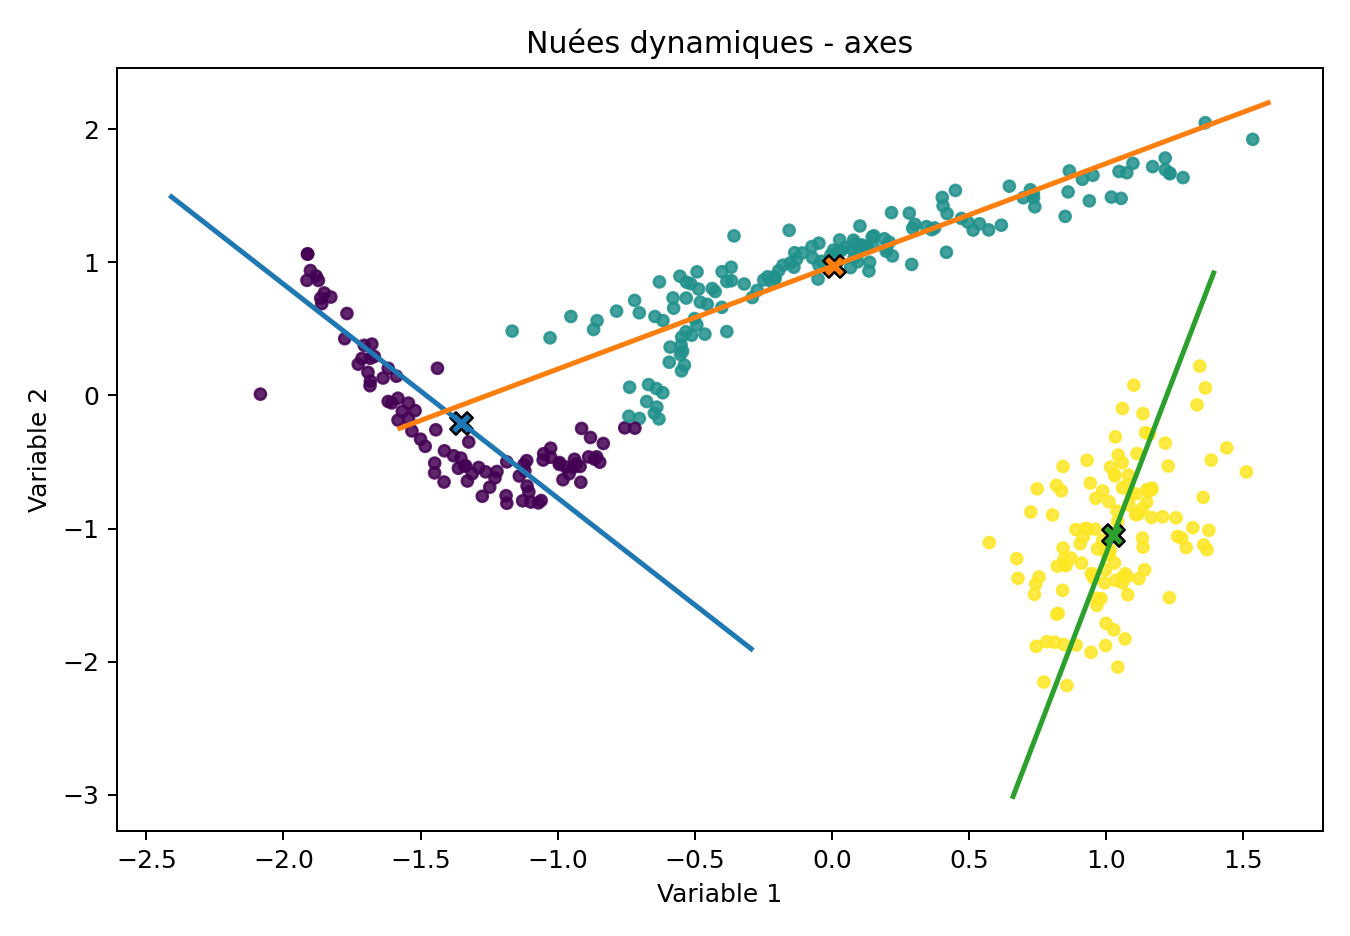
\includegraphics[width=0.72\textwidth]{figures/partition_axes.png}
\caption{Partition avec axes principaux. Source : calculs et visualisation de l'auteur.}
\end{figure}

\begin{figure}[H]
\centering
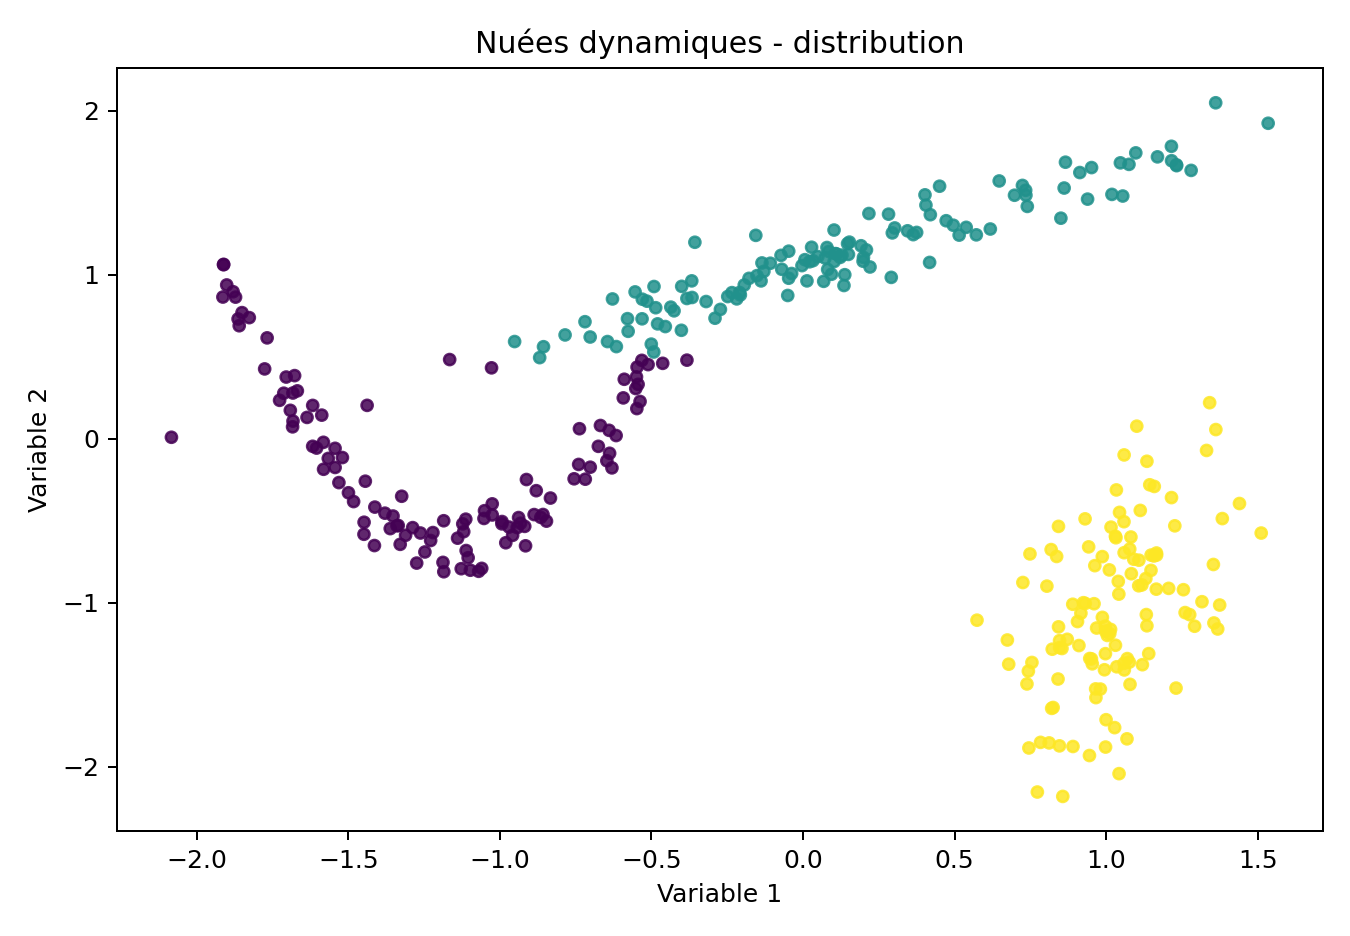
\includegraphics[width=0.72\textwidth]{figures/partition_distribution.png}
\caption{Partition avec représentation gaussienne. Source : calculs et visualisation de l'auteur.}
\end{figure}

\subsection{Interprétation}

L'interprétation suivante est tirée de nos résultats, en tenant compte de la nature des représentations documentées plus haut : le centroïde fournit une description ponctuelle conforme au mécanisme de k-means \cite{macqueen1967,lloyd1982} ; les prototypes multiples fournissent plusieurs ancrages dans la classe selon l'esprit des étalons de Diday \cite[p.~25]{diday1971} ; les axes décrivent des directions de variance selon l'ACP \cite{jolliffe2016} ; la covariance permet d'introduire une géométrie quadratique de type Mahalanobis \cite{mahalanobis1936} ; enfin, la médiane et la MAD donnent une description robuste de position et d'échelle \cite{rousseeuwcroux1993}.

La comparaison chiffrée entre ces cinq modes reste propre au jeu de données synthétique et aux paramètres choisis. \textit{Les conclusions quantitatives de cette sous-section sont donc des résultats de l'auteur, pas des résultats reproduits d'une publication.}

\section{Interface utilisateur}

L'interface et les commandes décrites dans cette section ont été développées spécifiquement pour le TP. Elles ne proviennent pas d'une source scientifique externe.

\subsection{Ligne de commande}

Exemple pour plusieurs prototypes :

\begin{lstlisting}
python app.py --representation points --clusters 3 \
              --n-representatives 7
\end{lstlisting}

Cas ponctuel :

\begin{lstlisting}
python app.py --representation point --clusters 3
\end{lstlisting}

Le programme produit \texttt{labels.csv}, \texttt{class\_costs.csv} et \texttt{summary.json}. Les formats de ces sorties sont des choix de conception de l'auteur.

\subsection{Interface Streamlit}

Une interface interactive permet de charger un CSV, de choisir $K$ et de sélectionner l'un des cinq types de représentation : point, ensemble de points, axes, distribution ou structure robuste. La commande de lancement est :

\begin{lstlisting}
streamlit run streamlit_app.py
\end{lstlisting}

Cette couche d'interface répond au cahier des charges du TP en rendant explicite le choix du type de nuée. \textit{La conception de l'interface est originale au projet.}

\section{Validation et tests}

Les tests automatisés fournis avec le dépôt ont été écrits pour vérifier le comportement du code : exécution des cinq représentations, production de $K$ classes non vides sur le jeu de test et cohérence de la prédiction dans un cas ponctuel simple. \textit{Ces tests sont des productions de l'auteur et ne sont pas issus d'une suite de tests externe.}

\begin{lstlisting}
pytest -q
\end{lstlisting}

Au moment de la génération de ce rapport, les deux tests présents dans le projet passent. Cette information provient de l'exécution locale du code et non d'une source bibliographique.

\section{Limites et améliorations possibles}

Diday suggère déjà d'examiner d'autres distances ou indices de similarité, et son article mentionne notamment l'utilisation de la distance euclidienne et d'autres mesures \cite[p.~24]{diday1971}. À partir de cette ouverture et de notre architecture, plusieurs améliorations sont envisageables : exécutions multiples avec différentes initialisations, ajout de nouvelles fonctions de distance, personnalisation des représentants, expérimentation sur des jeux de données réels et optimisation de la recherche de prototypes. \textit{Cette liste d'améliorations est une proposition de l'auteur, motivée par les limites observées dans le code.}

L'initialisation k-means++ peut aussi être étudiée plus systématiquement, puisque sa motivation est précisément de choisir avec davantage de soin les graines initiales \cite{arthur2007}. De même, les méthodes de médoïdes décrites par Kaufman et Rousseeuw offrent des pistes pour renforcer le raffinement des représentants réels \cite{kaufman1990}.

\section{Conclusion}

Le programme reprend le mécanisme central de la méthode de Diday : des classes sont définies relativement à des représentants, les observations sont affectées selon un coût, puis les représentants sont mis à jour de manière itérative \cite[pp.~20--23]{diday1971}. L'implémentation réalisée ici sépare volontairement ce moteur général de la nature précise du représentant.

Le mode ponctuel correspond à une mise à jour de type k-means \cite{macqueen1967,lloyd1982}. Les modes à plusieurs prototypes, axes, distribution gaussienne et structure robuste introduisent respectivement des idées appuyées sur les étalons de Diday \cite{diday1971}, la sélection de prototypes \cite{gonzalez1985,kaufman1990}, l'ACP \cite{jolliffe2016}, la distance quadratique de Mahalanobis \cite{mahalanobis1936} et la MAD \cite{rousseeuwcroux1993}. Les métriques de validation utilisées sont elles aussi référencées à leurs publications d'origine \cite{rousseeuw1987,hubert1985}.

La contribution propre du TP réside donc dans l'assemblage, l'implémentation \textit{from scratch}, l'interface commune, les choix de coûts pour les extensions et l'expérimentation reproductible. Cette séparation entre sources scientifiques et travail original rend le projet traçable et limite le risque de plagiat académique.

\begin{thebibliography}{99}

\bibitem{diday1971}
E. Diday,
\textit{Une nouvelle méthode en classification automatique et reconnaissance des formes : la méthode des nuées dynamiques},
Revue de Statistique Appliquée, vol. 19, no 2, pp. 19--33, 1971.
\url{http://www.numdam.org/item?id=RSA_1971__19_2_19_0}

\bibitem{macqueen1967}
J. MacQueen,
``Some Methods for Classification and Analysis of Multivariate Observations'',
in \textit{Proceedings of the Fifth Berkeley Symposium on Mathematical Statistics and Probability}, vol. 1, pp. 281--297, University of California Press, 1967.

\bibitem{lloyd1982}
S. P. Lloyd,
``Least Squares Quantization in PCM'',
\textit{IEEE Transactions on Information Theory}, vol. 28, no 2, pp. 129--137, 1982.
DOI: \href{https://doi.org/10.1109/TIT.1982.1056489}{10.1109/TIT.1982.1056489}.

\bibitem{arthur2007}
D. Arthur and S. Vassilvitskii,
``k-means++: The Advantages of Careful Seeding'',
in \textit{Proceedings of the Eighteenth Annual ACM-SIAM Symposium on Discrete Algorithms (SODA)}, pp. 1027--1035, 2007.
DOI: \href{https://doi.org/10.1145/1283383.1283494}{10.1145/1283383.1283494}.

\bibitem{gonzalez1985}
T. F. Gonzalez,
``Clustering to Minimize the Maximum Intercluster Distance'',
\textit{Theoretical Computer Science}, vol. 38, pp. 293--306, 1985.
DOI: \href{https://doi.org/10.1016/0304-3975(85)90224-5}{10.1016/0304-3975(85)90224-5}.

\bibitem{kaufman1990}
L. Kaufman and P. J. Rousseeuw,
\textit{Finding Groups in Data: An Introduction to Cluster Analysis},
Wiley, New York, 1990.
DOI: \href{https://doi.org/10.1002/9780470316801}{10.1002/9780470316801}.

\bibitem{jolliffe2016}
I. T. Jolliffe and J. Cadima,
``Principal Component Analysis: a Review and Recent Developments'',
\textit{Philosophical Transactions of the Royal Society A}, vol. 374, no 2065, art. 20150202, 2016.
DOI: \href{https://doi.org/10.1098/rsta.2015.0202}{10.1098/rsta.2015.0202}.

\bibitem{mahalanobis1936}
P. C. Mahalanobis,
``On the Generalised Distance in Statistics'',
\textit{Proceedings of the National Institute of Sciences of India}, vol. 2, no 1, pp. 49--55, 1936.

\bibitem{rousseeuwcroux1993}
P. J. Rousseeuw and C. Croux,
``Alternatives to the Median Absolute Deviation'',
\textit{Journal of the American Statistical Association}, vol. 88, no 424, pp. 1273--1283, 1993.
DOI: \href{https://doi.org/10.1080/01621459.1993.10476408}{10.1080/01621459.1993.10476408}.

\bibitem{rousseeuw1987}
P. J. Rousseeuw,
``Silhouettes: A Graphical Aid to the Interpretation and Validation of Cluster Analysis'',
\textit{Journal of Computational and Applied Mathematics}, vol. 20, pp. 53--65, 1987.
DOI: \href{https://doi.org/10.1016/0377-0427(87)90125-7}{10.1016/0377-0427(87)90125-7}.

\bibitem{hubert1985}
L. Hubert and P. Arabie,
``Comparing Partitions'',
\textit{Journal of Classification}, vol. 2, pp. 193--218, 1985.
DOI: \href{https://doi.org/10.1007/BF01908075}{10.1007/BF01908075}.

\bibitem{harris2020}
C. R. Harris, K. J. Millman, S. J. van der Walt, et al.,
``Array Programming with NumPy'',
\textit{Nature}, vol. 585, pp. 357--362, 2020.
DOI: \href{https://doi.org/10.1038/s41586-020-2649-2}{10.1038/s41586-020-2649-2}.

\end{thebibliography}

\appendix
\section{Commandes de reproduction}

\begin{lstlisting}[basicstyle=\ttfamily\footnotesize]
# Installer les dépendances
pip install -r requirements.txt

# Lancer une classification
python app.py --representation points --clusters 3 \
              --n-representatives 7

# Générer les expériences et les figures
python experiments/run_experiments.py

# Lancer l'interface
streamlit run streamlit_app.py

# Lancer les tests
pytest -q
\end{lstlisting}

\noindent\textit{Source : commandes propres au projet développé dans ce TP.}

\section{Extrait du cœur de l'algorithme}

L'extrait ci-dessous est issu du fichier \texttt{src/dynamic\_clouds.py} du projet. La boucle alternée est inspirée de la structure itérative de Diday \cite[p.~21]{diday1971}, mais le code lui-même est une implémentation originale du TP.

\begin{lstlisting}[basicstyle=\ttfamily\footnotesize]
for it in range(1, self.max_iter + 1):
    costs = self._cost_matrix(X, reps)
    new_labels = np.argmin(costs, axis=1)
    new_labels = self._repair_empty_clusters(X, new_labels, costs)
    objective = float(np.sum(costs[np.arange(len(X)), new_labels]))

    labels_unchanged = np.array_equal(new_labels, labels)
    labels = new_labels
    reps = self._fit_representatives(X, labels, rng)

    if labels_unchanged:
        break
\end{lstlisting}

\end{document}
